\section{Internal Tests}

\subsection{GOAL Test Set}
\label{5_internal_goal}
First of all, let us see how many unsuccessful complementation tasks there were with the internal tests on the \goal{} test set. Table~\ref{i.g.out_table} shows the number of timeouts and memory excesses for each of the eight tested versions of the Fribourg construction.

\begin{table}[ht]
\centering
% latex table generated in R 3.1.2 by xtable 1.7-4 package
% Sat Jun  6 16:42:17 2015
\begin{tabular}{lrr}
  \hline
Construction & Timeouts & Memory excesses \\ 
  \hline
Fribourg & 48 & 0 \\ 
  Fribourg+R2C & 30 & 0 \\ 
  Fribourg+R2C+C & 54 & 0 \\ 
  Fribourg+M1 & 2 & 0 \\ 
  Fribourg+M1+M2 & 1 & 0 \\ 
  Fribourg+M1+R2C & 1 & 0 \\ 
  Fribourg+M1+R2C+C & 8 & 0 \\ 
  Fribourg+R & 48 & 0 \\ 
   \hline
\end{tabular}

\caption{Number of timeouts and memory excesses in the internal tests on the \goal{} test set.}
\label{i.g.out_table}
\end{table}

As we can see in the table, there were no memory excesses, that is, none of the 11,000 complementation tasks required more than 1 GB memory (actually, Java heap size). On the other hand, there is quite a number of timeouts. If we extract the effective samples from these result sets, we get a set of 10,939 automata. That means that these 10,939 automata have been successfully completed by all the versions of the Fribourg construction, whereas the remaining 61 automata (0.55\%) provoked a timeout in at least one of the versions.

Our main analysis is now about the sizes of the complements of these 10,939 automata. With size we mean the number of states of an automaton. A stripchart as the one in Figure~\ref{i.g.stripchart} is a good way to get a first glance of the complement sizes. Each horizontal strip contains 10,939 dots, each one corresponding to a produced complement automaton. The x-position of a dot indicates the size of the corresponding complement automaton.

\begin{figure}[ht]
\centering
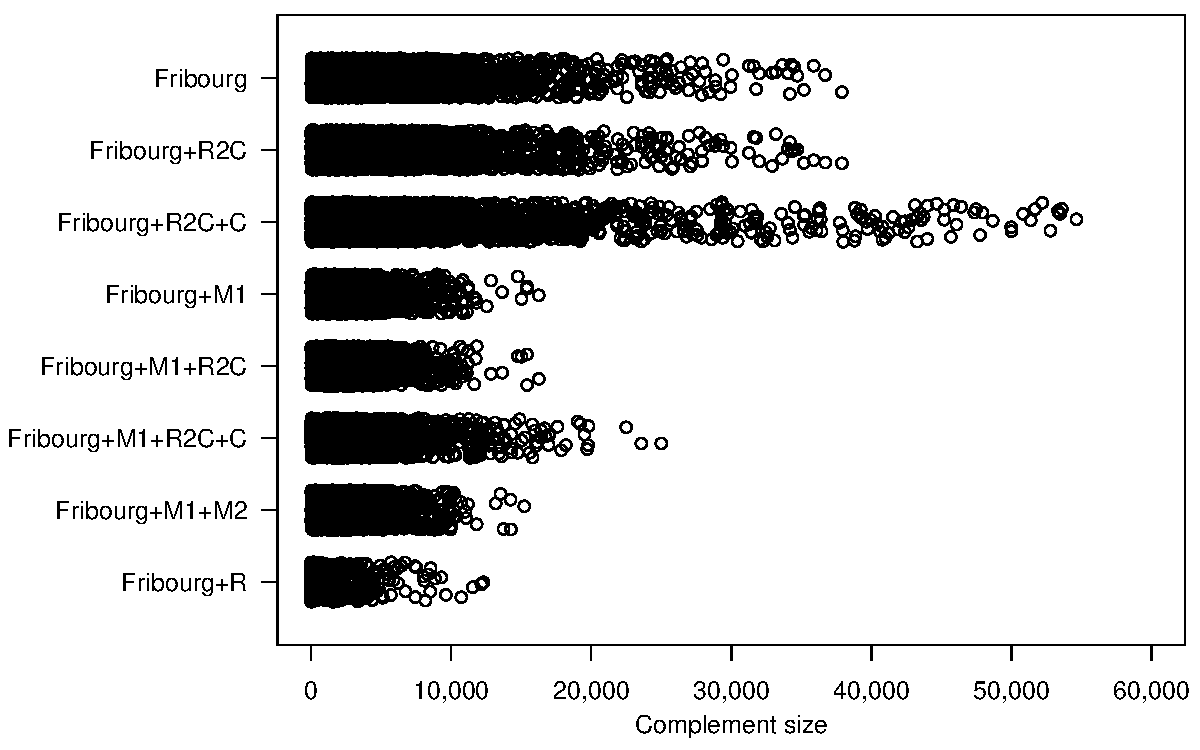
\includegraphics[width=0.7\textwidth]{figures/r/internal/goal/s.stripchart.pdf}
\caption{Stripchart with the complement sizes of the 10,939 effective samples of the \goal{} test set.}
\label{i.g.stripchart}
\end{figure}

The first thing to note is that the distribution of complement sizes is extremely right-skewed (also known as positive-skewed). The peak close to the left end of the x-axis and there is a long tail toward the right. This means that most of the complements are very small and the frequency decreases with increasing complement size. Finally, there are some few complements which are very large. This distribution implies that the mean is generally higher than the median, because the mean is ``dragged'' to the right by the few very large complements.

Next, we can compare the distributions of the individual version to each other. While Fribourg and Fribourg+R2C have a similarly long tail, Fribourg+R2C+C has a considerably longer one. This clearly is the effect of increasing the size of 91\% of the automata by adding a sink state in order to make them complete. Next, Fribourg+M1, Fribourg+M1+M2, and Fribourg+M1+R2C have similarly long tails that are significantly shorter than the ones of the previous versions. This indicates that the M1 optimisation is effective in reducing the size of otherwise large complements. Fribourg+M1+R2C+C, as expected, again increases the size of the tail due to the C option. Finally, Fribourg+R has a very short tail and an even higher concentration of very small complements. This is because the complements are pruned by removing their unreachable and dead states, and thus at least the complements of the 61.8\% universal input automata are reduced to empty automata of size 1.

Having a first impression of the distribution of complement sizes, we can look at some statistics characterising this distribution. Table~\ref{i.g.stats_table} shows the mean complement size along with the classic five-number summary consisting of minimum value, 25th percentile, median, 75th percentile and maximum value for each version of the Fribourg construction. As expected, the mean is always higher than the median. Generally, the median is a more robust metrics than the mean, because it is not affected by the value of outliers. This applies specifically to our distribution where some few very large complements might significantly increase the man whereas they leave the median unaffected. Therefore, the median will be our main metric, and the subsequent analyses will be based on the median.

\begin{table}[ht]
\centering
% latex table generated in R 3.1.2 by xtable 1.7-4 package
% Sat Jun  6 16:42:20 2015
\begin{tabular}{lrrrrrr}
  \hline
Construction & Mean & Min. & P25 & Median & P75 & Max. \\ 
  \hline
Piterman+EQ+RO & 209.6 & 1 & 38.0 & 80.0 & 183.0 & 20,349 \\ 
  Slice+P+RO+MADJ+EG & 949.4 & 2 & 120.0 & 396.0 & 1,003.0 & 41,081 \\ 
  Fribourg+M1+R2C & 1,017.3 & 2 & 153.0 & 452.0 & 1,134.0 & 37,068 \\ 
   \hline
\end{tabular}

\caption{Statistics of the complement sizes of the 10,939 effective samples of the \goal{} test set.}
\label{i.g.stats_table}
\end{table}

Going through the median values in Table~\ref{i.g.stats_table} we encounter some surprises. To begin with, as expected, there is a decrease from Fribourg (761) to Fribourg+R2C (689). Then, however, there is a significant drop to 451 with Fribourg+R2C+C. This is a surprise insofar as by looking at Figure~\ref{i.g.stripchart}, Fribourg+R2C+C seems to have the worst performance at a first glance. Indeed it also has the highest mean, which is due to the group of extremely large complements. The median, however, is very low, even lower than the one of Fribourg+M1 with its significantly shorter tail in Figure~\ref{i.g.stripchart}. Also the 25th percentile of Fribourg+R2C+C is with 85 one of the lowest. Going to the other side of the median, however, the 75th percentile (2,329) is the largest of all versions. A possible characterisation of this phenomenon is that the C option (together with R2C) makes small complements smaller, and large complements larger. The diminishment of small complements is far-reaching enough that the median is affected by it and decreased significantly.

The next thing we see in Table~\ref{i.g.stats_table} is that the median of Fribourg+M1 (482) is slightly lower than the median of Fribourg+M1+M2 (496). The same applies to the 25th and 75th percentile. This backs up our statement from Section~\ref{4_internal} that Fribourg+M1 performs better on the \goal{} teset set than Fribourg+M1+M2. The difference is rather small (the median increase is by 2.9\%), but it is enough to consider Fribourg+M1 as the better of the two versions, and to combine it therefore with R2C and R2C+C.

Fribourg+M1+R2C brings down the median from 482 to 447, with respect to Fribourg+M1. Also the 25th and 75th percentile are decreased. Adding the C option to Fribourg+M1+R2C, again causes the median to drop dramatically, from 447 to 331. The 25th percentile decreases from 152 to 83. The 75th percentile however increases from 1,118 to 1,208.5. Here we have again the same picture of the effecto of adding the C option that we had before. Namely that small complements are made smaller, and large complements are made larger.

Finally, the last row in Table~\ref{i.g.stats_table} with Fribourg+R shows the extent of unreachable and dead states that the Fribourg construction produces. The median is 1, and a further analysis reveals that the single-state complements go up to the 61st percentile. That is, 61\% of the complements have a size of 1. This is likely to correspond to the 61.8\% of universal automata in the GOAL test set whose complements can be reduced to empty automata with a single state.

% Time
% \begin{table}[ht]
% \centering
% % latex table generated in R 3.1.2 by xtable 1.7-4 package
% Wed Aug 19 09:24:28 2015
\begin{tabular}{LrrrrrrRr}
  \hline
Construction & Mean & Min. & P25 & Median & P75 & Max. & Total & $\approx$ hours \\ 
  \hline
Fribourg & 8.5 & 2.5 & 3.3 & 4.9 & 7.3 & 586.0 & 93,351.2 & 259 \\ 
  Fribourg+R2C & 6.6 & 2.2 & 2.9 & 4.2 & 6.4 & 219.7 & 72,545.7 & 202 \\ 
  Fribourg+R2C+C & 8.5 & 2.2 & 2.6 & 3.5 & 6.4 & 582.9 & 93,396.2 & 259 \\ 
  Fribourg+M1 & 4.9 & 2.5 & 3.2 & 4.1 & 5.9 & 55.1 & 54,061.3 & 150 \\ 
  Fribourg+M1+R2C & 4.4 & 2.2 & 2.8 & 3.6 & 5.3 & 42.5 & 48,572.0 & 135 \\ 
  Fribourg+M1+R2C+C & 5.6 & 2.5 & 3.2 & 4.0 & 6.5 & 147.4 & 60,918.9 & 169 \\ 
  Fribourg+M1+M2 & 4.6 & 2.2 & 2.9 & 3.8 & 5.1 & 38.4 & 49,848.0 & 138 \\ 
  Fribourg+R & 7.5 & 2.2 & 3.0 & 3.9 & 6.3 & 470.5 & 82,387.3 & 229 \\ 
   \hline
\end{tabular}

% \caption{Running times in seconds of the complementation tasks, measured as CPU time.}
% \end{table}
% \textcolor{red}{It is strange that Fribourg+R is so much faster than Fribourg}

Up to now, we only looked at statistics aggregated over the entire test set. But as we know from Section~\ref{4_goal_testset}, the 11,000 automata of the \goal{} test set are divided into 110 classes which consist of combinations of 11 transition densities and 10 acceptance densities. The transition densities range from 1 to 3 in steps of 0.2, and the acceptance densities range from 0.1 to 1 in steps of 0.1. In each class there are 100 automata. It is assumable that the median complement sizes are different for different classes. In the next step of the analysis, we want to analyse exactly this point. How do the median complement sizes of the different classes compare to each other, and can we identify a pattern of the classes that result in large and small complements?

This type of analysis naturally results in three-dimensional data. The classes themselves have two dimensions (the transition densities and the acceptance densities), and each of them has a third dimension consisting of the median complement size of this class. One way to present such data is by, for example, a 11x10 matrix with the rows being the transition densities, the columns the acceptance densities, and the cells the median values. Another way is by so called perspective plots. We used both of these ways in Section~\ref{4_goal_testset} when we analysed the number of complete and universal automata in each class of the \goal{} test set. In the present analysis, we will use perspective plots and omit the matrices for space reasons. However, we present the corresponding matrices in Appendix~\ref{app_matrices}. In this way, the interested reader may consult the exact values of the median complement sizes for each class. In the same way, we restrict ourselves to the median complement sizes as the third dimension. The same analysis could also be done, for example, for the mean, the 25th percentile, or the 75th percentile of complement sizes. However, as mentioned, we consider the median to be the most meaningful statistics, and thus exclusively focus on it for the matter of conciseness.

Figures~\ref{i.g.persp-1} and~\ref{i.g.persp_2} show the perspective plots of the median complement sizes for the 110 classes of the \goal{} test set. Each crossing of two lines on the xy-plane represents a class, and the z-value (height) of thie crossing indicates the median complement size of this class. As a help for the orientation, if one imagines the corresponding matrices, as they are presented in Appendix~\ref{app_matrices}, then in the perspective plots we are looking at these matrices from the bottom-right corner. That is, the class that is in the top-left corner of a matrix (transiton density 1.0 and acceptance density 0.1) is the one that is the farthest away from the viewer in the corresponding perspective plot. This orientation holds for all the remaining perspective plots in this thesis. The colours of the squares in the perspective plot (called facets) are a function of the z-values of their four corners and are selected to draw an analogy with topographical terrain maps.

\newcommand{\perspwidth}{0.475}

\begin{figure}[ht]
\centering
  \hfill
  \begin{subfigure}[t]{\perspwidth\textwidth}
  \centering
  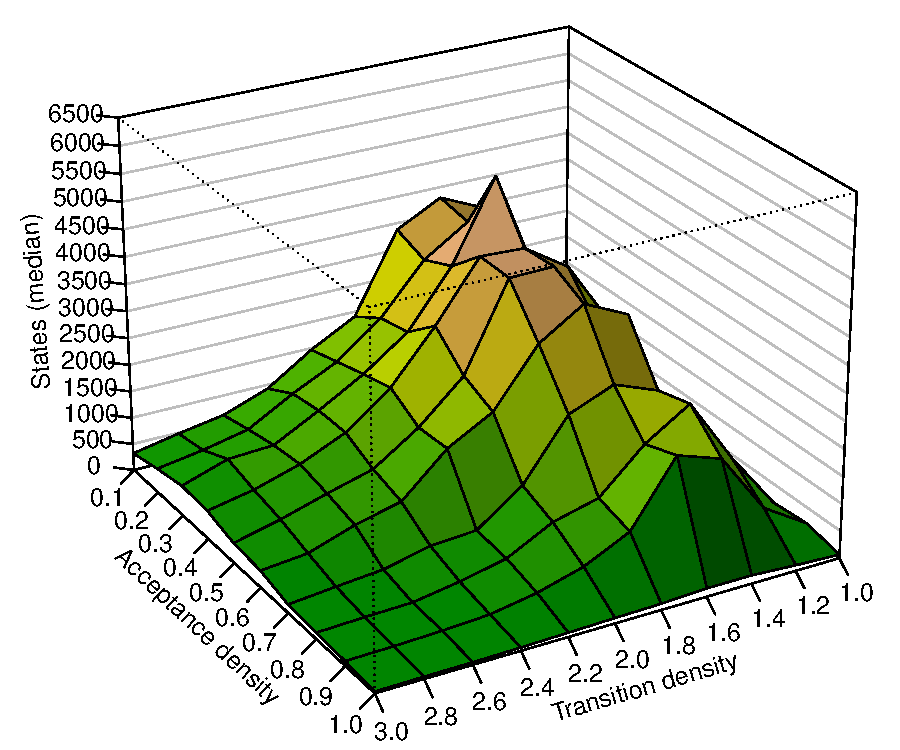
\includegraphics[width=\textwidth]{figures/r/internal/goal/s.median.Fribourg.pdf}
  \caption{Fribourg}
  \end{subfigure}
  \hfill
  \begin{subfigure}[t]{\perspwidth\textwidth}
  \centering
  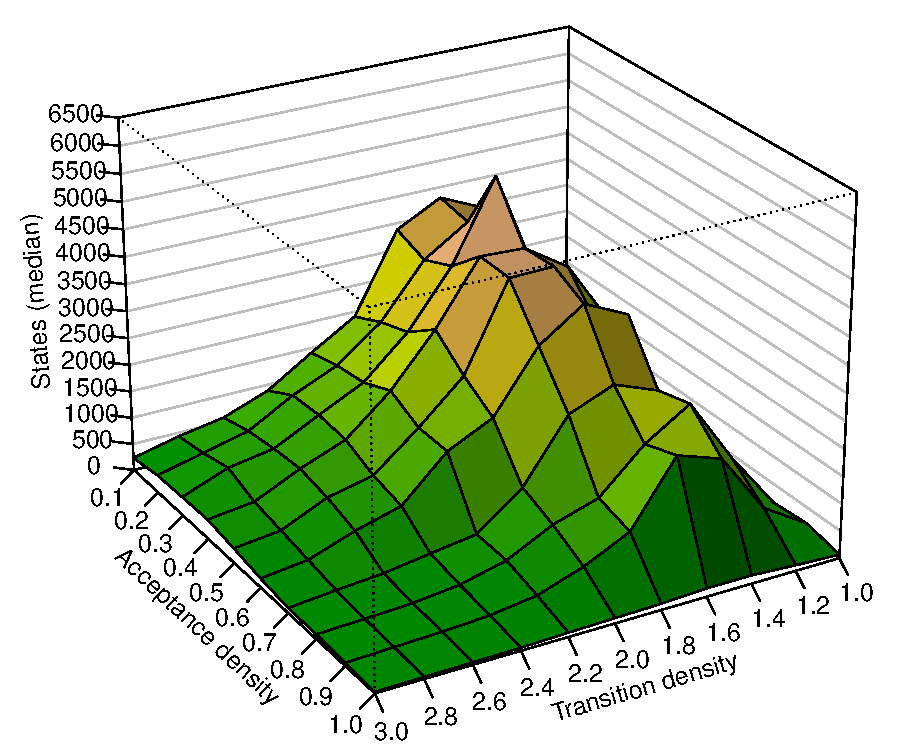
\includegraphics[width=\textwidth]{figures/r/internal/goal/s.median.Fribourg+R2C.pdf}
  \caption{Fribourg+R2C}
  \end{subfigure}
  \hfill

  \hfill
  \begin{subfigure}[t]{\perspwidth\textwidth}
  \centering
  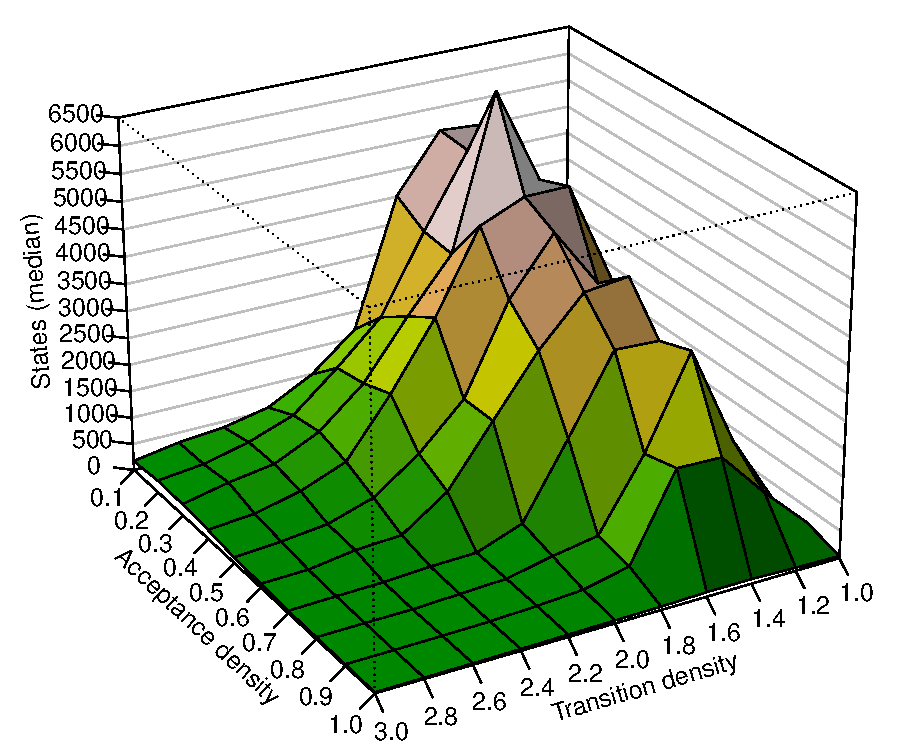
\includegraphics[width=\textwidth]{figures/r/internal/goal/s.median.Fribourg+R2C+C.pdf}
  \caption{Fribourg+R2C+C}
  \end{subfigure}
  \hfill
  \begin{subfigure}[t]{\perspwidth\textwidth}
  \centering
  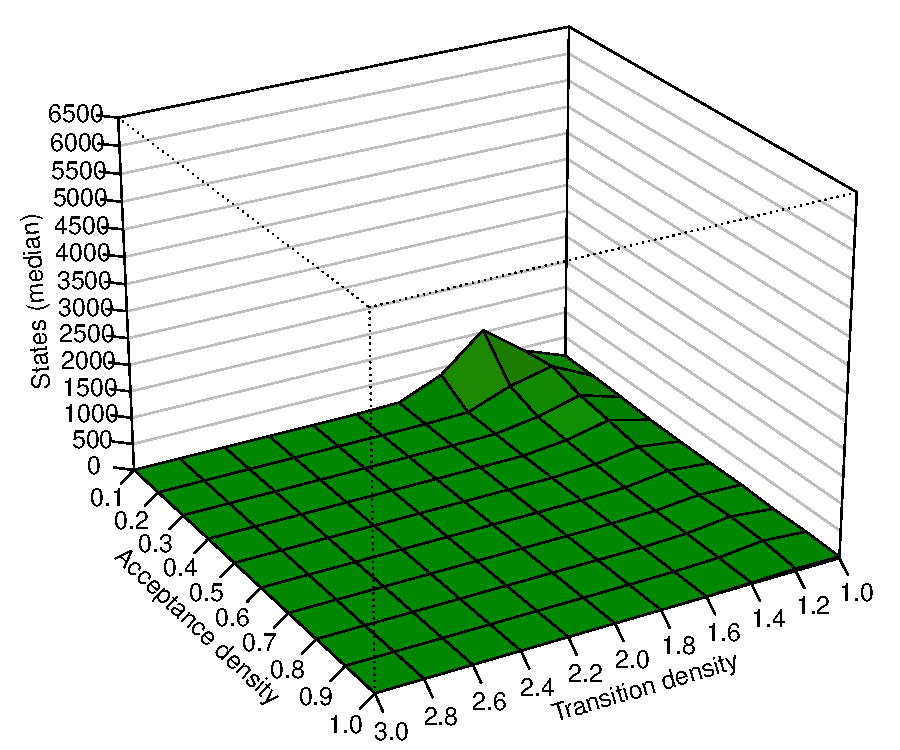
\includegraphics[width=\textwidth]{figures/r/internal/goal/s.median.Fribourg+R.pdf}
  \caption{Fribourg+R}
  \end{subfigure}
  \hfill  
\caption{Median complement sizes of the 110 transition density/acceptance density classes of the 10,939 effective samples of the \goal{} test set.}
\label{i.g.persp_1}
\end{figure}

The first thing we notice when looking at the plots in Figure~\ref{i.g.persp_1} and~\ref{i.g.persp_2} is that there are indeed large differences in the median complement sizes across the transition/acceptance density classes. Figuratively speaking, there is an oblong mountain (or hill) in the northern part of the area in east-west orientation, whose ridge increases in height from east to west and stays high until the western edge of the area. The mountain is located roughly in the area of transition densities between 1.2 and 2.2 and acceptance densities from 0.1 up to 0.9. This means that the automata of these classes are apparently harder to complement than the automata of other classes, as they result more frequently in larger complements.

We will further elaborate on the reasons of these different complement sizes across classes, and also try to characterise easy, medium, and hard automata for the Fribourg construction, at the end of this subsection. For now, we focus on the relative differences of median complement sizes between the different versions of the Fribourg construction.

Looking at Figure~\ref{i.g.persp_1}, the perspective plots for Fribourg and Fribourg+R2C are rather similar. The top of the mountain ridge is at between 3,500 and 4,000 states with a single peak of around 4900 states in the class with transition density 1.6 and acceptance density 0.3. From Table~\ref{i.g.stats_table} we can learn that the overall median complement size is 761 for Fribourg and 689 for Fribourg+R2C. These low values might surprise at first as the mountain, which is much higher, seems to dominate. However, by taking a closer look, it becomes apparent that around half of the classes are in rather low terrain (less than 1,000 states). Furthermore, the heights of the mountain peak do not allow to deduce anything about the overall median, because the median is not affected by the actual values of the data points which are greater than the median. This is the main characteristics of the median and applies to all the subsequent perspective plots in this chapter. The means in turn are 2,004.6 for Fribourg and 1955.9 for Fribourg+R2C.

Fribourg+R2C+C in Figure~\ref{i.g.persp_1} (c) has an even considerably higher mountain than the previous two versions. The top of the ridge is at around 5,000 states and the peak at the class with transition density 1.6 and acceptance density 0.3 has close to 6,500 states. This increase in height is however not reflected in the overall median of Fribourg+R2C+C relative to Fribourg+R2C. As we have seen in in Table~\ref{i.g.stats_table}, the median of Fribourg+R2C+C is 451, and thus 34.5\% lower than the median of Fribourg+R2C. By taking a closer look at the perspective plots, the reason for this can be seen, as the low areas of Fribourg+R2C+C are indeed slightly lower than the low areas of Fribourg+R2C. The significantly higher high areas of Fribourg+R2C+C do not have an effect on the overall median. However, they do have an effect on the overall mean which with 2,424.6 is indeed 24\% higher than the one of Fribourg+R2C (1,955.9).

Going from the first three perspective plot in Figure~\ref{i.g.persp_1} to the perspective plot of Fribourg+R is like going from the Swiss Alps to a Dutch polder. The mountain shrinks to a small hillock and the rest of the terrain is low and flat. This is because so many complements of the Fribourg construction can be reduced to very small sizes by removing their unreachable and dead states. A look at the corresponding matrix in Appendix~\ref{app_matrices} reveals that 68 of the 110 classes have a median complement size of 1. If we further compare this matrix to the matrix with the number of universal automata in Figure~\ref{4_compl_univ} (b), we see that all the classes with a median of 1 contain more than 50 universal automata, and the classes with a median greater than 1 contain less than 50 universal automata. There is a total of 100 automata per class. This makes sense as the complements of universal automata are empty automata, and every empty automaton can be reduced to an automaton with a single non-accepting state. Looking at the classes with a median greater than 1, we see that their values are still considerably lower than the ones of the plain Fribourg construction, which indicates that the Fribourg construction generates a large number of unreachable and dead states. However, as already mentioned, this thread of analysis is not the focus of the present thesis, and we leave it for future work.

\begin{figure}[ht]
\centering
  \hfill
  \begin{subfigure}[t]{\perspwidth\textwidth}
  \centering
  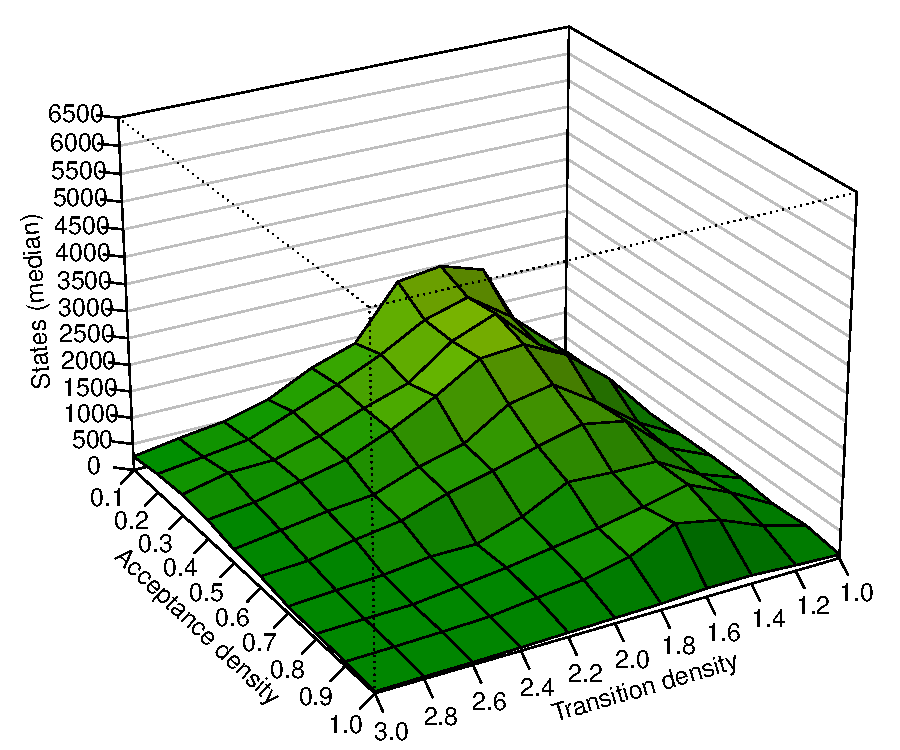
\includegraphics[width=\textwidth]{figures/r/internal/goal/s.median.Fribourg+M1.pdf}
  \caption{Fribourg+M1}
  \end{subfigure}
  \hfill
  \begin{subfigure}[t]{\perspwidth\textwidth}
  \centering
  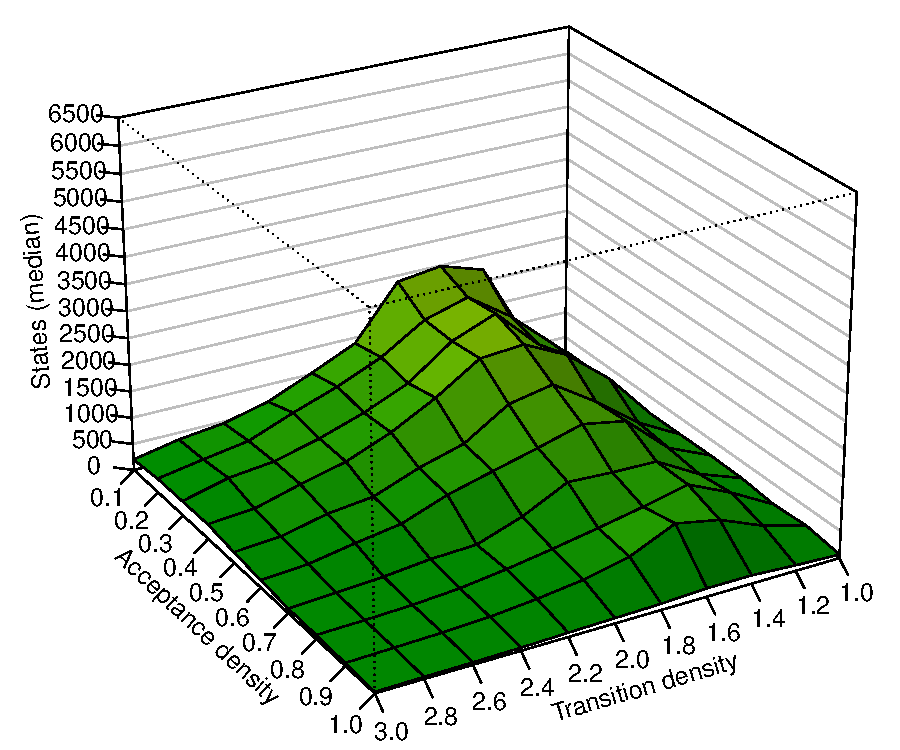
\includegraphics[width=\textwidth]{figures/r/internal/goal/s.median.Fribourg+M1+R2C.pdf}
  \caption{Fribourg+M1+R2C}
  \end{subfigure}
  \hfill

  \hfill
  \begin{subfigure}[t]{\perspwidth\textwidth}
  \centering
  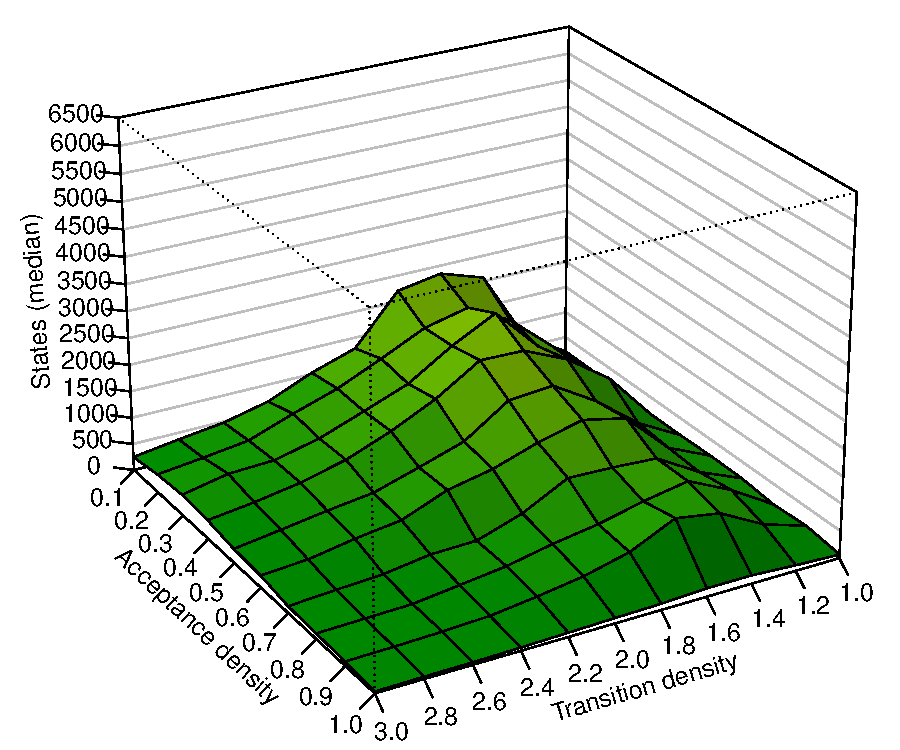
\includegraphics[width=\textwidth]{figures/r/internal/goal/s.median.Fribourg+M1+M2.pdf}
  \caption{Fribourg+M1+M2}
  \end{subfigure}
  \hfill
  \begin{subfigure}[t]{\perspwidth\textwidth}
  \centering
  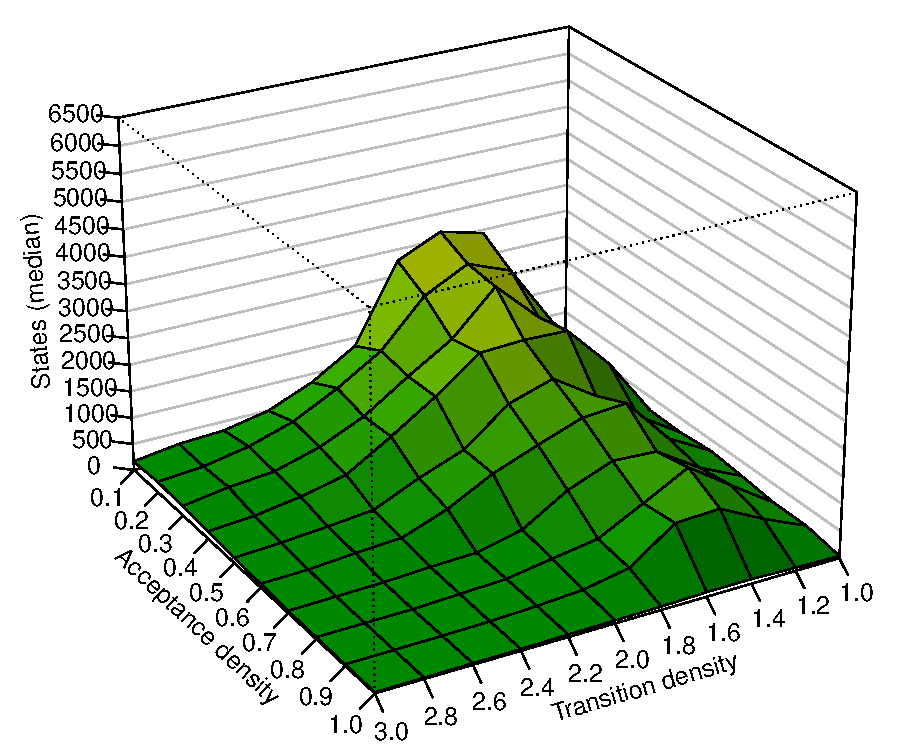
\includegraphics[width=\textwidth]{figures/r/internal/goal/s.median.Fribourg+M1+R2C+C.pdf}
  \caption{Fribourg+M1+R2C+C}
  \end{subfigure}
  \hfill
\label{i.g.persp_2}
\end{figure}

Figure~\ref{i.g.persp_2} shows the perspective plots of the remaining four versions of the Fribourg construction, all of which include the M1 optimisation. The first thing we note is that, while the mountain is still there, its height shrinks significantly. For Fribourg+M1, and Fribourg+M1+R2C, the top of the ridge is between is around 2,500 states. This is reflected by the overall means of these two versions compared to their counterparts without the M1 optimisation, Fribourg, and Fribourg+R2C. The decrease of the overall mean from Fribourg to Fribourg+M1 is by 52\% (from 2004.6 to 963.2) and from Fribourg+R2C to Fribourg+M1+R2C by 52.1\% (from 1955.9 to 937.7). The decreases of the overall medians are by 36.6\% (from 761 to 482), and 35.1\% (from 689 to 447) for the same two pairs of versions. With this we can confirm that the M1 optimisation brings a significant performance gain. 

Regarding the M2 optimisation, we can see that the mountain ridge in the Fribourg+M1+M2 perspective plot is slightly lower than the one in the Fribourg+M1 perspective plot. The flatland regions, however, seem to not change much. This is reflected by the overall mean of Fribourg+M1+M2 which is slightly lower than in Fribourg+M1 (958.9 opposed to 963.2). The overall median, on the other hand, is higher for Fribourg+M1+M2 than for Fribourg+M1 (496 opposed to 482). An interpretation of this behaviour is that the application of the M2 optimisation results in smaller complements for \textit{some} input automata. These automata are especially the ``hard'' ones that produce large complements. This positive effect of M2 does however not affect enough input automata, especially not the ``easy'' automata, as to improve the overall performance of the construction in terms of median complement size. As already stated previously, we consider therefore Fribourg+M1 as the better construction on the \goal{} test set than Fribourg+M1+M2.

Finally,Fribourg+M1+R2C+C differs from Fribourg+M1+R2C in a similar way Fribourg+R2C+C differs from Fribourg+R2C. The higher regions get higher and the lower regions get lower, that is, a performance decline on ``hard'' automata, but a performance gain on easy automata. The performance gain on the easy automata is however effective enough to decrease the overall median from 447 to 331, which is minus 26\%.

With 331 states, Fribourg+M1+R2C+C has the lowest median of all the versions (except Fribourg+R which is a special case because it modifies the output of the construction). However, we still declare Fribourg+M1+R2C as the winner on the \goal{} test set, mainly for two reasons. First, while Fribourg+M1+R2C+C has a lower median, the mean is still higher (1062.6 to 937.7 which is a plus of 13.3\%). This results from the complements of the hard automata, which are larger than with Fribourg+M1+R2C. From a practical point of view, the mean might be relevant, because it relates more directly to the required computing resources than the median. For example the execution CPU time per complementation task, that we also measured along with our experiments, is 25.4\% higher for Fribourg+M1+R2C+C than for Fribourg+M1+R2C. The increase in the average execution time per automaton is from 4.44 to 5.57 seconds and in the total execution time from 48,572 seconds ($\approx$ 135 hours) to 60,919 seconds ($\approx$ 169 hours). Fribourg+M1+R2C, on the other hand, has the lowest mean of all versions. The second reason that we choose Fribourg+M1+R2C as the winner and not Fribourg+M1+R2C+C is that the C option is not a real part of the construction. It actually modifies the input automata before the construction starts in order to make them better suited for the construction. Fribourg+M1+R2C, on the other hand, includes only native options, and input and output of the construction are not modified. This should also make it fairer to compare the Fribourg construction to other constructions in the external tests (Section~\ref{ext}).

As we have seen, there are big difference in the complement sizes across the different classes of the \goal{} test set. Furthermore, there is a certain pattern, namely the mountain in the north-western region of the class matrix. Automata of classes that are in the mountain region seem to be harder to complement than automata from the classes in the flatland region. We attempted to categorise the classes of the \goal{} test set into the three groups ``easy'', ``medium'', and ``hard''. To do so, we first averaged the matrices with the median complement sizes of all the eight versions of the Fribourg construction. In this way, we have a mean median complement size for each class. Then we defined two breakpoints that divide the classes into easy, medium, and hard groups. The breakpoints 500 and 1,600 result in an appropriate groups that seem to capture the reality well. The result with these breakpoints can be seen in Figure~\ref{i.g.difficulty}.

\begin{figure}[ht]
\centering
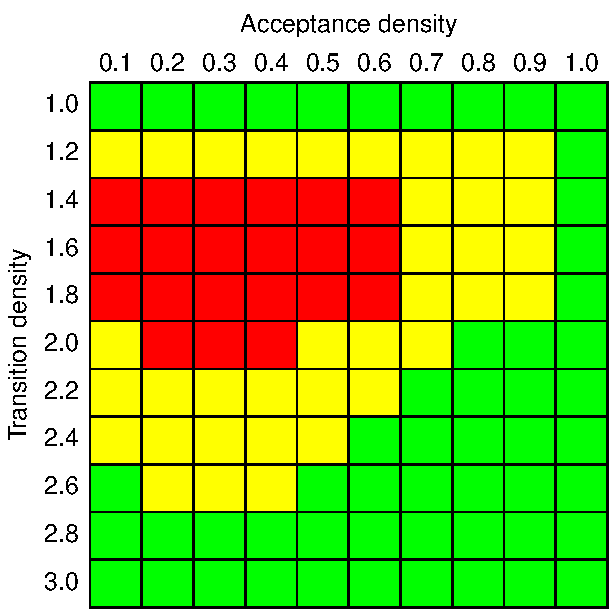
\includegraphics[width=0.35\textwidth]{figures/r/internal/goal/difficulty.pdf}
\caption{Difficulty categories of the transition/acceptance density classes of the \goal{} test set. Green: easy; yellow: medium; red: hard.}
\end{figure}

As can be seen in Figure~\ref{i.g.difficulty}, there are 53 easy, 36 medium, and 21 hard classes. The easy classes are mainly those with extreme values. In particular, all the classes with a low or high transition density of 0.1, or 2.8 and 3.0, and a high acceptance density of 1.0 are easy. Furthermore, there is a ``triangle'' of easy classes between transition densities 2.0 and 2.6. and acceptance densities 0.5 and 0.9. The higher the transition density, the lower the acceptance density may be so that the corresponding class is still easy. The hard classes are roughly those with a transition density between 1.4 and 1.8 and an acceptance density between 0.1 and 0.6. The medium classes finally are situated as a ``belt'' around the hard classes.

It is interesting that the extreme values of transition density and acceptance density result in easy automata. With a transition density of 1.0 and an alphabet size of 2, each of the 15 states has on average two outgoing and two incoming transitions\footnote{The transition density multiplied with the number of states defines the number of transition for each symbol of the alphabet in the automaton, see Section~\ref{4_goal_testset}.}. With a transition density of 3.0, each state has on average 6 outgoing and 6 incoming transitions. These low or high connectivity seems to considerably simplify the complementation task. The same applies to a high acceptance density of 1.0, which means that every state is an accepting state\footnote{The acceptance density defines the percentage of states that are accepting, see Section~\ref{4_goal_testset} as well.}. Generally, we can say that automata with high acceptance densities are easier to complement than automata with lower acceptance densities. This also means that the pattern of easy automata at the extreme values of transition and accceptance density, does not apply to to the lower extreme of the acceptance density. Automata with a very low acceptance density of 0.1 are hard to complement---unless they are made easy by a low or high transition density.

Another interesting point is that the hard automata have transition densities between 1.4 and 1.8. It seems that this range of transition densities is the crucial factor in the hardness of a complementation task, and that it is only alleviated by a growing acceptance density. This explains the decline of the mountain ridge from west to east.

Summarising we can say that transition densities between 1.4 and 1.8 produce the hardest complementation tasks, and that to the both sides the difficulty steadily decreases with declining or growing transition density. Furthermore, a growing acceptance density generally implies easier complementation tasks.


\subsection{Michel Test Set}
\label{5_internal_michel}
Our second test set consists of the four Michel automata with $m=\{1,\dots,4\}$ that are listed in Figure~\ref{4_michel_automata}. They have 3, 4, 5, and 6 states, respectively. Our main motivation to use these automata is to test our complementation construction on very difficult automata. In this way we can get an idea about the worst-case state complexity of our construction.

We complemented the four Michel automata with the six versions of the Fribourg construction which are listed in Section~\ref{4_internal}. We did not impose a time or memory limitation for the individual complementation tasks, as we wanted every task to finish. The resulting complement sizes are listed in Table~\ref{i.m.states}.

\begin{table}[htb]
\centering
% latex table generated in R 3.1.2 by xtable 1.7-4 package
% Sun Aug 16 00:19:45 2015
\begin{tabular}{lrrrrrr}
  \hline
Construction & Michel 1 & Michel 2 & Michel 3 & Michel 4 & Fitted curve & Std. error \\ 
  \hline
Fribourg & 57 & 843 & 14,535 & 287,907 & $(1.35n)^n$ & 0.01\% \\ 
  Fribourg+R2C & 33 & 467 & 8,271 & 168,291 & $(1.24n)^n$ & 0.06\% \\ 
  Fribourg+M1 & 44 & 448 & 5,506 & 81,765 & $(1.10n)^n$ & 0.07\% \\ 
  Fribourg+M1+M2 & 42 & 402 & 4,404 & 57,116 & $(1.03n)^n$ & 0.12\% \\ 
  Fribourg+M1+M2+R2C & 28 & 269 & 3,168 & 43,957 & $(0.99n)^n$ & 0.04\% \\ 
  Fribourg+R & 18 & 95 & 528 & 3,315 & $(0.64n)^n$ & 0.35\% \\ 
   \hline
\end{tabular}

\caption{Complement sizes of the Michel automata with $m=\{1,\dots,4\}$ and 3, 4, 5, and 6 states, respectively. }
\label{i.m.states}
\end{table}

In the second-last column ``Fitted curve'' of Table~\ref{i.m.states}, we fitted a function of the form $(an)^n$ to the measured data points of the previous four columns. These data points consist of the sizes of the four Michel automata (3, 4, 5, and 6) as. The fitted function $(an)^n$ can be seen as an approximated generalisation of the state growth, where $n$ is the size of the input automaton. The last colum ``Std. error'' shows the standard error that resulted from the fit of the previous column.

We can see in Table~\ref{i.m.states} that the state growths are indeed very large. For example, complementing Michel~4, which has six states, with the plain Fribourg construction results in a complement of 287,907 states. However, the optimisations R2C, M1, and M2 have a large influence on the complement sizes. If we consider Michel~4, then the R2C optimisation alone reduces the complement size from 287,907 to 168,291 which is a reduction of 51.5\%. The M1 optimisation has an eve larger influence as it reduces the complement size from 287,907 to 81,765 which is a reduction of 71.6\%. Adding M2 to M1 further reduces the complement size of Fribourg+M1 by 30.1\% (from 81,765 to 57,116). Finally, adding R2C on top of M1 and M2 brings a further reduction of of 23\% (from 57,116 to 43,957). If we compare the most efficient version (Fribourg+M1+M2+R2C) with the least efficient one (Fribourg), then the three optimisations reduce the complement size by 85.7\%, or in other words, the complement size of Fribourg+M1+M2+R2C is 15.3\% of the complement size of Fribourg.

It is interesting to see that for the Michel automata Fribourg+M1+M2 is more efficient than Fribourg+M1. For the \goal{} test set, Friburg+M1+M2 had a slighly higher overall median than Fribourg+M1 although it had a slightly lower overall mean. We identified in Section~\ref{5_internal_goal} that the M2 optimisation has a positive effect only on some automata, and that these are mostly the hard automata. Michel automat are very hard automata, and indeed the M2 optmisation has a considerably positive effect. These results support thus the observation we made in Section~\ref{5_internal_goal}.

The special version Fribourg+R yields very small complements compared to the other versions. This tells us that the complements of the other versions contain a large number of unreachable and dead states. For example, the complement of Michel~4 of Fribourg+R (3,315 states) is 1.2\% of the size of the complement of Fribourg. This means that 98.8\% of the 287,907 states of the complement of Fribourg are unreachable and dead states. This is actually not surprising, because, following the proof of Michel~\cite{michel1988}\cite{1996_thomas}, the smallest possible complement of Michel~4 has 24 states. This is because Michel~4 has $m=4$ and Michel proved that the complement has at least size $m!$. This means that that the Fribourg construction is very far from reaching these optimal complement sizes.

Up to now we just looked at the specific results of Michel~4. The fitted functions of the form $(an)^n$ summarise the results of all the four Michel automata. These functions give us reference points for the worst-case state complexities of the different versions of the Fribourg construction. For example, for the plain Fribourg construction with its fitted function of $(1.35n)^n$, we know now empirically that this construction produces complements of size $(1.35n)^n$, where $n$ is the size of the input automaton. This means that the real (theoretical) worst-case complexity cannot be lower than $(1.35n)^n$ (but it can still be higher). This bound decreases for the different versions of the Fribourg construction until $(0.99n)^n$ for Fribourg+M1+M2+R2C. This value is still greater than the lower bound of $(0.76n)^n$ for Büchi complementation determined by Yan~\cite{2006_yan}.

We also measured the execution times for the individual complementation tasks. This time was measured in CPU time, that is, the time the task is running on the CPU. Table~\ref{i.m.times} shows the measured values in seconds. We can see that the difference between the least and most efficient version is bigger than for the complement sizes. For example for Michel~4, Fribourg+M1+M2+R2C is more than 43 times faster than Fribourg (2,332.6 seconds compared to 100,976 seconds). In more familiar unities, this corresponds to approximately 39 minutes for Fribourg+M1+M2+R2C against 28 hours for Fribourg. We also fitted functions of the form $(an)^n$ to the measured execution times where $n$ is the number of states of the input automaton, and the value of the function is the execution time of the taks in CPU time seconds.

\begin{table}[htb!]
\centering
% latex table generated in R 3.1.2 by xtable 1.7-4 package
% Sun Aug 16 16:21:25 2015
\begin{tabular}{lrrrrrr}
  \hline
Construction & Michel 1 & Michel 2 & Michel 3 & Michel 4 & Fitted curve & Std. error \\ 
  \hline
Piterman+EQ+RO & 2.5 & 3.8 & 42.6 & 75,917.4 & $(1.08n)^n$ & 0.64\% \\ 
  Slice+P+RO+MADJ+EG & 2.3 & 3.6 & 11.4 & 159.5 & $(0.39n)^n$ & 0.38\% \\ 
  Rank+TR+RO & 2.2 & 3.0 & 6.4 & 30.0 & $(0.29n)^n$ & 0.18\% \\ 
  Fribourg+M1+M2+R2C & 2.5 & 3.5 & 10.8 & 2,332.6 & $(0.61n)^n$ & 0.62\% \\ 
   \hline
\end{tabular}

\caption{Execution times.}
\label{i.m.times}
\end{table}

The fitted functions that we calculated for the measured complement sizes and execution times are based on four data points and basically only valid for the first four Michel automata. They can thus not be used to reliably extrapolate values for larger Michel automata. However, it is still interesting to do such an extrapolation in order to see the involved complexity and to show why we were restricted to include only the first four Michel automata in the test set. In Table~\ref{i.m.extrapolation}, we show extrapolated values for the complement sizes and execution times for the plain Fribourg construction (the least efficient one), based on the corresponding fitted functions. The table includes the values for the Michel automat 5 to 8, which have 7 to 10 states. 


\begin{table}[htb]
\centering
\begin{tabular}{lrrr}
\hline
Automaton & Compl. size $(1.35n)^n$ & Exec. time $(1.14n)^n$ & $\approx$ days/months/years \\
\hline
Michel 5 &       6,882,980 &      2,020,385 &     23 days \\
Michel 6 &     189,905,394 &     46,789,245 &     18 months \\
Michel 7 &   5,939,189,262 &  1,228,250,634 &     39 years \\
Michel 8 & 207,621,228,081 & 36,039,825,529 &  1,142 years \\
\hline
\end{tabular}
\caption{Extrapolated values for the complement sizes and execution times for the Michel automata with $m=\{5,\dots,10\}$ with the plain Fribourg construction.}
\label{i.m.extrapolation}
\end{table}

According to the fitted state growth function, the complement of Michel~5 would have nearly 7 million states, and the complement of Michel~8 even more than 207 billions. Already the computation of the 7 million states of Michel~5 would most probably exceed the available memory resources in our computing environment. Regarding the extrapolated exeution times, the complementation of Michel~5 would take 23 days. This would similarly exceed the maximum running time of a job on the computer cluster on which we executed the computations. And even without these restriction, at least starting from Michel~6, the exectuion times between 18 months and 1,142 years are clearly too long to be included in a master's thesis.




\section{External Tests}
\label{5_external}
In the external tests we compare the results of the most efficient version of the Fribourg construction to the results of three pre-implemented constructions in \goal. These constructions are Piterman+EQ+RO, Slice+P+RO+MADJ+EG, and Rank+TR+RO. The most efficient version of the Fribourg construction differs for the two test sets. For the \goal{} test set it is Fribourg+M1+R2C, and for the Michel test set it is Fribourg+M1+M2+R2C. In the following two sections we present the results of all these constructions on the two test sets.


\subsection{GOAL Test Set}
\label{5_external_goal}
For the \goal{} test set we compared Fribourg+M1+R2C with Piterman+EQ+RO, Slice+P+RO+MADJ+EG, and Rank+TR+RO. As for the internal tests, we set a time limit of 600 seconds CPU time, and a memory limit determined by a Java heap size of 1 GB per complementation task. If a task does not finish within these limits, it is aborted and marked as either a timed out or memory exceeded. Table~\ref{e.g.outs} shows the number of timeouts and memory excesses that we observed for the four constructions.


\begin{table}[ht]
\centering
% latex table generated in R 3.1.2 by xtable 1.7-4 package
% Sat Jun  6 16:42:17 2015
\begin{tabular}{lrr}
  \hline
Construction & Timeouts & Memory excesses \\ 
  \hline
Fribourg & 48 & 0 \\ 
  Fribourg+R2C & 30 & 0 \\ 
  Fribourg+R2C+C & 54 & 0 \\ 
  Fribourg+M1 & 2 & 0 \\ 
  Fribourg+M1+M2 & 1 & 0 \\ 
  Fribourg+M1+R2C & 1 & 0 \\ 
  Fribourg+M1+R2C+C & 8 & 0 \\ 
  Fribourg+R & 48 & 0 \\ 
   \hline
\end{tabular}

\caption{Number of timeouts and memory excesses.}
\label{e.g.outs}
\end{table}

Most striking in Table~\ref{e.g.outs} is the high number of unsuccessful tasks for the Rank construction. 3,317 of the 11,000 automata (33.8\%) were aborted due to a timeout, and further 83 (0.8\%) due to a memory excess. Regarding the other constructions, there are just two timeouts for the Piterman, and one timeout for the Fribourg construction.

Determining the effective samples of these runs gives a number of 7,204 automata (65.5\%). In Figure~\ref{e.g.stripchart.with_rank} we present the complement sizes of these 7,204 effective samples as a stripchart. Looking at this picture makes the reason for the high number of aborted tasks of the Rank construction apparent. Rank+TR+RO produces a very big number of very large complements compared to the other constructions. 

\begin{figure}[ht]
\centering
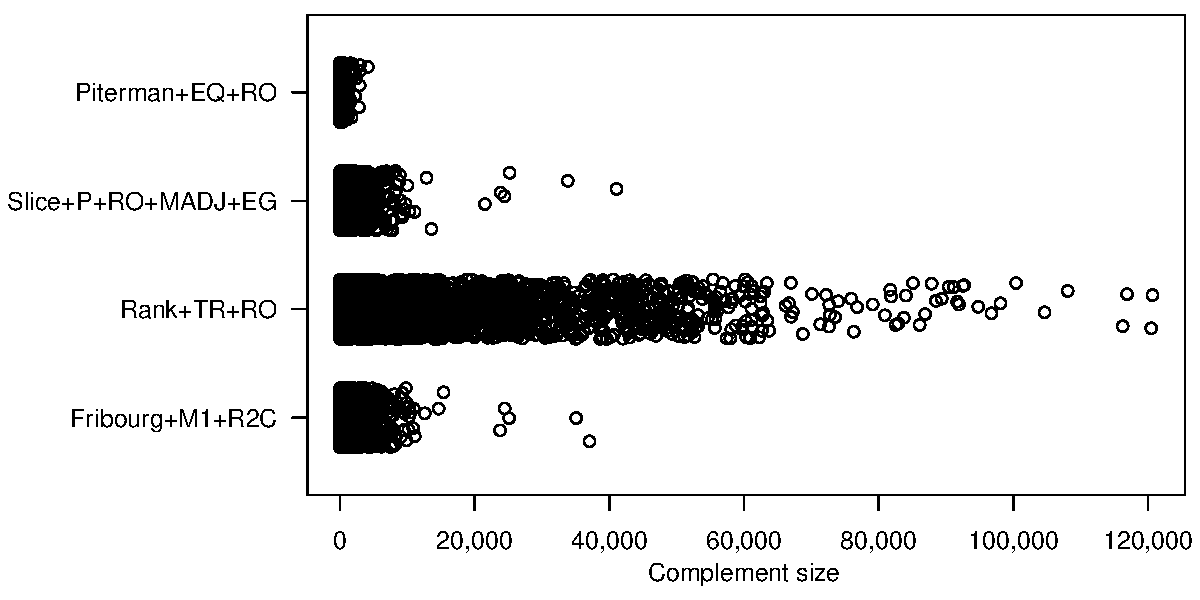
\includegraphics[width=0.75\textwidth]{figures/r/external/goal/s.stripchart.with_rank.pdf}
\caption{Complement sizes of the 7,204 effective samples.}
\label{e.g.stripchart.with_rank}
\end{figure}

But from the stripchart in Figure~\ref{e.g.stripchart} alone we cannot yet tell whether the Rank construction \textit{generally} produces larger complements than the other constructions, or if this holds just for \textit{some} automata. Therefore, we calculated further statistics of the complement sizes of the 7,204 effective samples in Table~\ref{e.g.stats.with_rank}. 

\begin{table}[ht]
\centering
% latex table generated in R 3.1.2 by xtable 1.7-4 package
% Sun Aug 16 15:57:19 2015
\begin{tabular}{lrrrrrr}
  \hline
Construction & Mean & Min. & P25 & Median & P75 & Max. \\ 
  \hline
Piterman+EQ+RO & 106.0 & 1 & 29.0 & 58.0 & 121.0 & 4,126 \\ 
  Slice+P+RO+MADJ+EG & 555.4 & 2 & 70.0 & 202.0 & 596.0 & 41,081 \\ 
  Rank+TR+RO & 5,255.6 & 2 & 81.0 & 254.5 & 3,178.2 & 120,674 \\ 
  Fribourg+M1+R2C & 662.9 & 2 & 101.0 & 269.0 & 754.5 & 37,068 \\ 
   \hline
\end{tabular}

\caption{Aggregated statistics of complement sizes of the 7,204 effective samples.}
\label{e.g.stats.with_rank}
\end{table}

And indeed, the 25th percentile and the median of Rank are higher than for Piterman and Slice, but still lower than for our Fribourg construction. However, the picture changes dramatically for the 75th percentile where the value of Rank is more than four times higher than the value for Fribourg. Also the mean of Rank is many times higher than the means of all the other constructions. A possible explanation for this is that the Rank construction performs comparably with the other constructions on easy automata. For the one half of easier automata of the 7,204 effective samples, Rank performs even better than our Fribourg construction, as shown by the median values. For harder automata, however, the performance of Rank is decreased tremendously, and the construction results in very large complements that are beyond any comparison wihth the complements of the other constructions. In addition, the automata that are hardest for Rank are not even included in this analysis. These are the 34.5\% of the test set that Rank could not complete within the given resource restrictions. If we would have these results and include them in the analysis, then the picture would probably look even much more distorted.

What we cannot tell is whether the automata which are hard for Rank are the same that are hard for the other constructions. However, as we will see later, we think that this is not necessarily the case.

Given the large number of unsuccessful complementation tasks of Rank we decided to do the main analysis and comparison of the results without the Rank construction. Because with the Rank construction would basically exclude more than one third of the taks that have been successfully completed by the other constructions from the result analysis. Our main interest is to compare the performance of the Fribourg construction to the other constructions. Above we have already compared it to the special behaviour of the Rank construction, and by excluding Rank from the further analysis, we can compare the Fribourg constructions in full detail with the Piterman and Slice constructions.

Without Rank there are 10,998 effective samples, that is, there are only two automata that have not been completed by all the three of Piterman, Slice, and Fribourg. In Figure~\ref{e.g.stripchart} we display the complement sizes of these 10,998 effective samples as a stripchart.

\begin{figure}[ht]
\centering
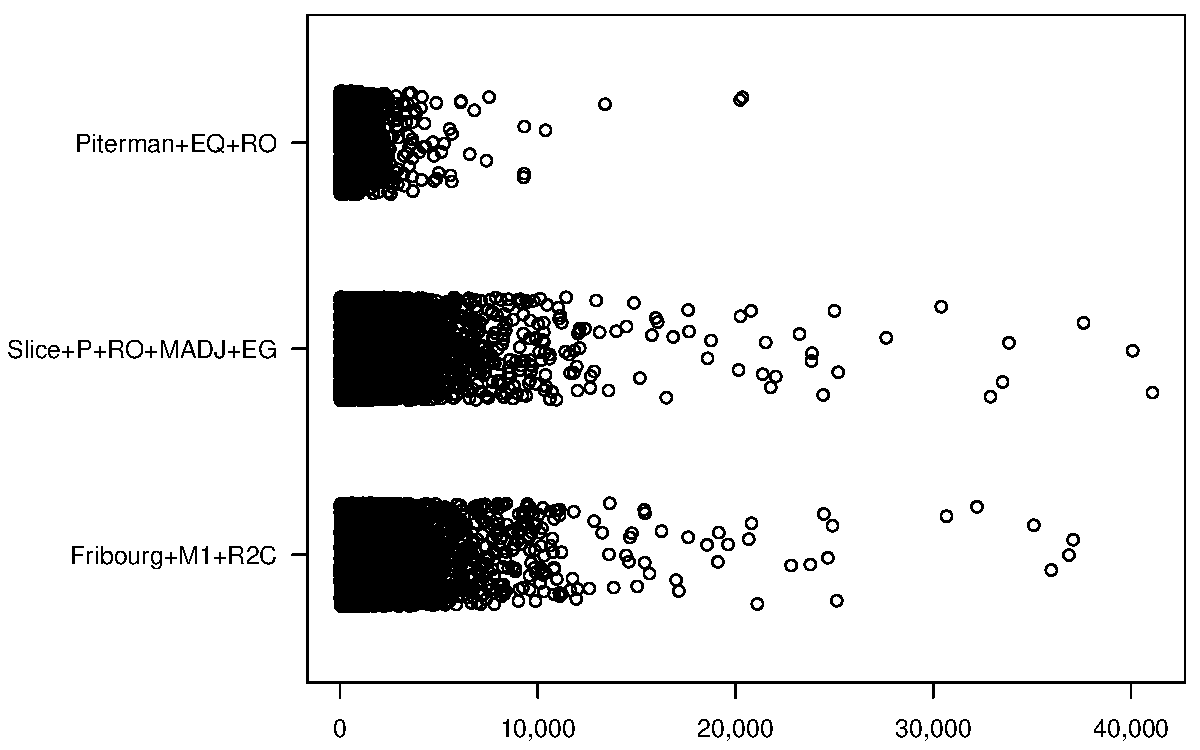
\includegraphics[width=0.75\textwidth]{figures/r/external/goal/s.stripchart.pdf}
\caption{Complement sizes of the 10,998  effective samples.}
\label{e.g.stripchart}
\end{figure}

From the stripchart we can see that Fribourg and Slice have a comparable distribution of complement sizes, whereas Piterman has a considerably higher concentration of small complement sizes. We can say that Piterman generally produces smaller complement than Fribourg and Slice.

We present the statistics of these distributions in Table~\ref{e.g.stats}. 
Indeed, for all statistics Piterman has values that are in the order of magnitudes lower than the ones of Fribourg and Slice. It is interesting that this order of magnitude for the mean, 25th percentile, median, and 75th percentile is very roughly five. It seems that Piterman produces throughout complements that are around five times smaller than the complements of Fribourg and Slice.


\begin{table}[ht]
\centering
% latex table generated in R 3.1.2 by xtable 1.7-4 package
% Sat Jun  6 16:42:20 2015
\begin{tabular}{lrrrrrr}
  \hline
Construction & Mean & Min. & P25 & Median & P75 & Max. \\ 
  \hline
Piterman+EQ+RO & 209.6 & 1 & 38.0 & 80.0 & 183.0 & 20,349 \\ 
  Slice+P+RO+MADJ+EG & 949.4 & 2 & 120.0 & 396.0 & 1,003.0 & 41,081 \\ 
  Fribourg+M1+R2C & 1,017.3 & 2 & 153.0 & 452.0 & 1,134.0 & 37,068 \\ 
   \hline
\end{tabular}

\caption{Aggregated statistics of complement sizes of the 10,998 effective samples without Rank.}
\label{e.g.stats}
\end{table}

Comparing Fribourg and Slice, there is a slight favour for Slice. Mean, 25th percentile, median, and 75th percentile are lower for Slice than for Fribourg by 6.7\%, 21.6\%, 12.4\%, and 11.6\%, respectively. We have to conclude that from an overall point of view, the Fribourg construction has the second-worst performance for the \goal{} test set after Piterman and Slice, and before Rank.

But now let us look at the results for the 110 classes of transition density and acceptance density classes of the \goal{} test set. As already for the internal tests, we take the median complement size as our statistic of interest and calculate it for each of the 110 classes. The results as perspective plots are shown in Figure~\ref{e.g.persp}. The same data in matrix form can be found in Appendix~\ref{app_matrices}.

\renewcommand{\perspwidth}{0.3}
\begin{figure}[ht]
\centering
  \hfill
  \begin{subfigure}[t]{\perspwidth\textwidth}
  \centering
  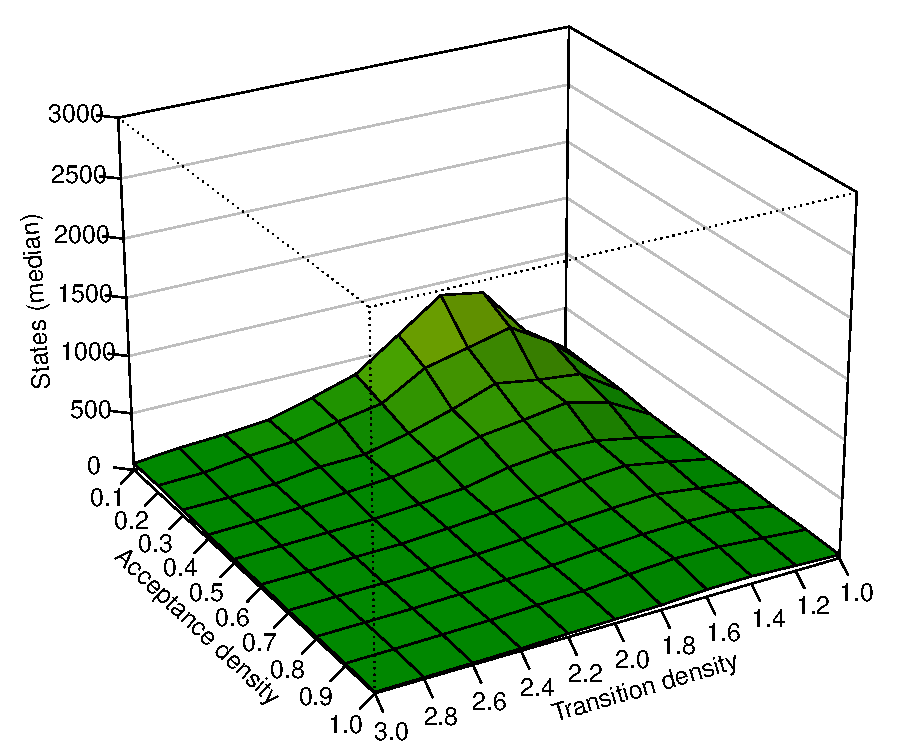
\includegraphics[width=\textwidth]{figures/r/external/goal/s.median.Piterman+EQ+RO.pdf}
  \caption{Piterman+EQ+RO}
  \end{subfigure}
  \hfill
  \begin{subfigure}[t]{\perspwidth\textwidth}
  \centering
  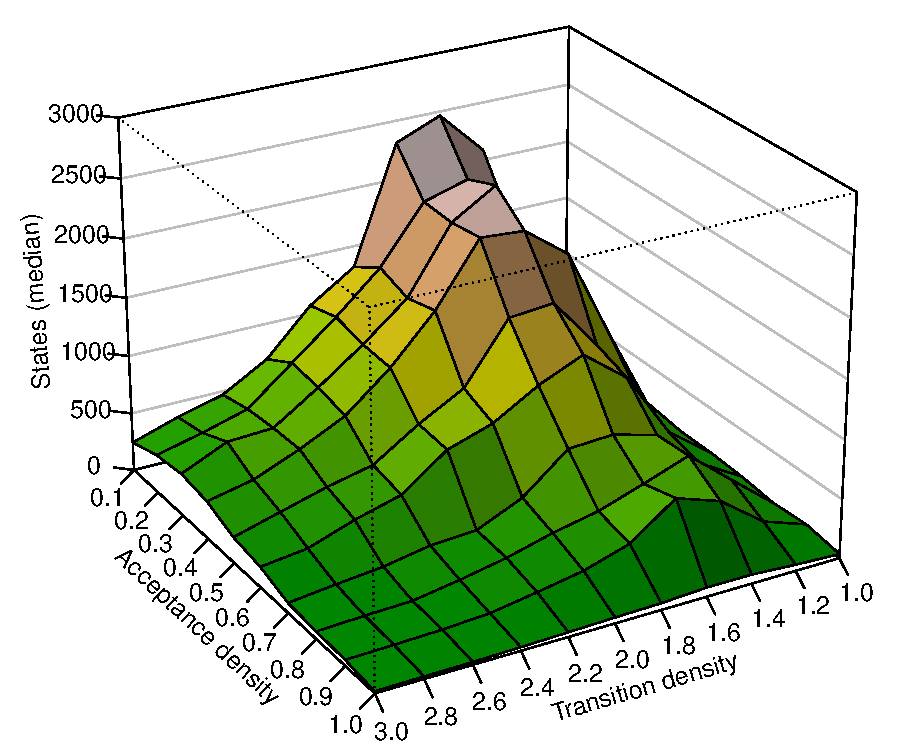
\includegraphics[width=\textwidth]{figures/r/external/goal/s.median.Slice+P+RO+MADJ+EG.pdf}
  \caption{Slice+P+RO+MADJ+EG}
  \end{subfigure}
  \hfill
  \begin{subfigure}[t]{\perspwidth\textwidth}
  \centering
  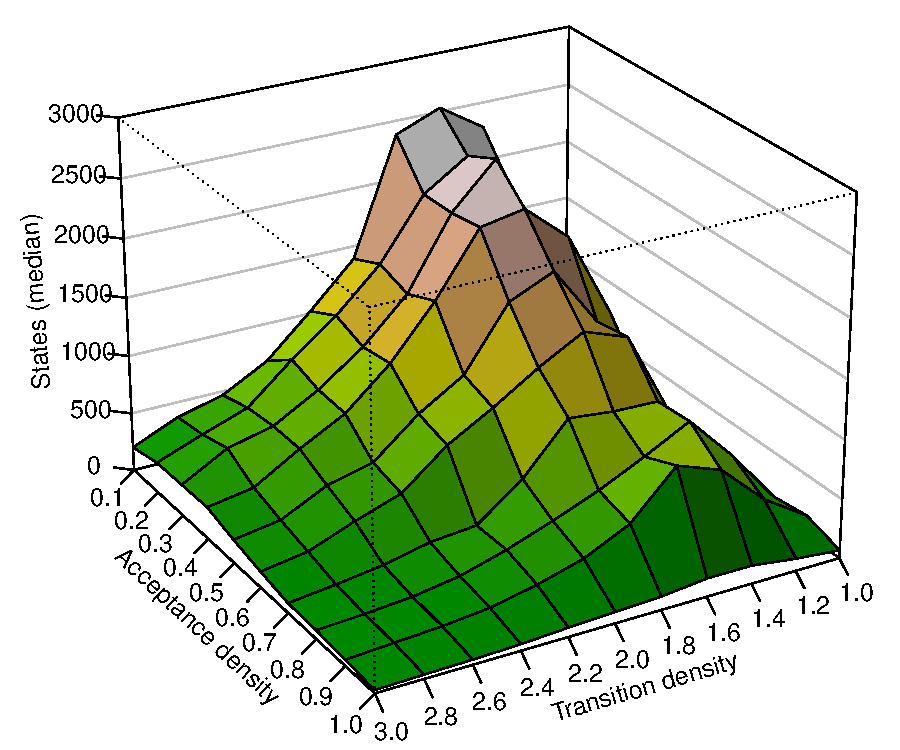
\includegraphics[width=\textwidth]{figures/r/external/goal/s.median.Fribourg+M1+R2C.pdf}
  \caption{Fribourg+M1+R2C}
  \end{subfigure}
  \hfill
\caption{Median complement sizes (10,998 samples)}
\label{e.g.persp}
\end{figure}

First of all, note that the data displayed in the perspective plot of Fribourg+M1+R2C in Figure~\ref{e.g.persp} (c) is the same as the one from the internal tests in in Figure~\ref{i.g.persp_2} (b). The only difference is the range of the $z$-axis, which in Figure~\ref{i.g.persp_2} ranges from 0 to 6,500, and in Figure~\ref{e.g.persp} from 0 to only 3,000.

We can see that the pattern for Fribourg and Slice are very similar. The median complement sizes in the individual classes do not differ a lot, both relatively and absolutely. However, the medians of Fribourg seem to be throughout (with some exceptions) slightly higher than the ones of Slice. This means that Fribourg and Slice seem to have similar strengths and weaknesses, but Slice is slightly more efficient on the tested automata.

Piterman, as expected, has medians that are throughout multiple times lower than the corresponding medians of Fribourg and Slice. The basic pattern, however, is still similar. There is a mountain ridge along the classes with a transition density of 1.6 with its top in the class with transition density 1.6 and acceptance density 0.1. Thus, this supports our claim from before that throughout all of the tested automata, Piterman produces complements that are multiple times smaller than the corresponding ones of Fribourg and Slice.

\subsection{Michel Automata}
\label{5_external_michel}
We tested the same three third-party constrcutions, Piterman+EQ+RO, Slice+P+RO+MADJ+EG, and Rank+TR+RO on the Michel automata 1 to 4 and compared the results with the version of the Friboug construction that was most efficient on the Michel automata in the internal tests. This version is Fribourg+M1+M2+R2C. As for the internal tests, we did not set a time or memory limitation as we wanted every task to successfully finish.

The resulting complement sizes are shown in Table~\ref{e.m.states}. Again, we fitted a function of the form $(an)^n$ to the four measured data points of each construction and calculated the standard error of this fit.

\begin{figure}[ht]
\centering
% latex table generated in R 3.1.2 by xtable 1.7-4 package
% Sun Aug 16 00:19:45 2015
\begin{tabular}{lrrrrrr}
  \hline
Construction & Michel 1 & Michel 2 & Michel 3 & Michel 4 & Fitted curve & Std. error \\ 
  \hline
Fribourg & 57 & 843 & 14,535 & 287,907 & $(1.35n)^n$ & 0.01\% \\ 
  Fribourg+R2C & 33 & 467 & 8,271 & 168,291 & $(1.24n)^n$ & 0.06\% \\ 
  Fribourg+M1 & 44 & 448 & 5,506 & 81,765 & $(1.10n)^n$ & 0.07\% \\ 
  Fribourg+M1+M2 & 42 & 402 & 4,404 & 57,116 & $(1.03n)^n$ & 0.12\% \\ 
  Fribourg+M1+M2+R2C & 28 & 269 & 3,168 & 43,957 & $(0.99n)^n$ & 0.04\% \\ 
  Fribourg+R & 18 & 95 & 528 & 3,315 & $(0.64n)^n$ & 0.35\% \\ 
   \hline
\end{tabular}

\caption{Complement sizes of the first four Michel automata.}
\label{e.m.states}
\end{figure}

Considering the results of the \goal{} test set, the results in Table~\ref{e.m.states} are surprising. Rank is the most efficient construction. It produces the smallest complements for all Michel automata, and with $(0.91n)^n$ it has the flattest fitted curve of all constructions. This is surprising because for the \goal{} test set, Rank produced by far the largest complements, and 34.5\% of the test data could not even be completed within the given time and memory limits. With the Michel automata, however, the case seems to be reversed and Rank produces by far the smallest complements.

Rank is followed by the Fribourg construction, which has the second-smallest complements for Michel~3 and~4, and with $(0.99n)^n$ the second-flattest fitted curve. The complements of Michel~2, 3, and~4 of the Fribourg construction are bigger than the ones of the Rank construction by 48.6\%, 68.2\%, and 69.2\%, respectively. With this, our Fribourg construction is relatively close to the clear winner, which is the Rank construction.

The next in the ranking is the Slice construction with a fitted curve of $(1.18n)^n$. for Michel~1 to~3, this is actually the worst construction, but then for Michel~4, the complement is smaller than the one of Piterman what results in the flatter fitted curve. The gap to the second-ranked construction, Fribourg, is big. The complement sizes of Michel~2 to~4 exceed the ones of Fribourg by 60.2\%, 114.2\%, and 180.2\%, respectively. This is also a remarkable point, because for the \goal{} test set, Fribourg and Slice showed a very similar performance.

The last in the ranking is Piterman with a fitted curve of $(1.25n)^n$. However, special for Piterman is that it has the smallest complement for Michel~1 (together with Rank), the second-smallest for Michel~2, the third-smallest for Michel~3, and the largest for Michel~4. It is actually the large complement of Michel~4 that makes Piterman having the steepest fitted curve. However, it is still remarkable that the construction which is by far the most efficient on the \goal{} test set produces so much worse results for the Michel automata than all the other constructions. Compared with the Rank construction, Piterman's complements of Michel~2 to~4 are 38.7\%, 174.3\%, and 573.6\%, respectively, bigger. And this is exactly the Rank construction that performed so much worse on the \goal{} test set that it made a comparison with the Piterman construction nearly impossible. Compared to the Fribourg construction, Piterman produces slightly smaller complements for Michel~1 and~2, but larger ones for Michel~3 and~4. Namely, they are 63.1\% and 298.2\% larger than the corresponding ones of the Fribourg construction.

Summarising we can say that the ranking of the constructions for the Michel test set is exactly the reverse of the ranking for the \goal{} test set. The by far worst construction for the \goal{} test set (Rank) is the best one for the Michel test set, and the by far best construction for the \goal{} test set (Piterman) is the worst one for the Michel test set (at least for Michel~4). For the Fribourg construction this means that it ``advances'' from rank 3 of 4 for the \goal{} test set to rank 2 of 4 for the Michel test set.

We also measured the execution times of the individual complementation tasks in CPU time seconds. The results are shown in Table~\ref{e.m.times}.

\begin{table}[ht]
\centering
% latex table generated in R 3.1.2 by xtable 1.7-4 package
% Sun Aug 16 16:21:25 2015
\begin{tabular}{lrrrrrr}
  \hline
Construction & Michel 1 & Michel 2 & Michel 3 & Michel 4 & Fitted curve & Std. error \\ 
  \hline
Piterman+EQ+RO & 2.5 & 3.8 & 42.6 & 75,917.4 & $(1.08n)^n$ & 0.64\% \\ 
  Slice+P+RO+MADJ+EG & 2.3 & 3.6 & 11.4 & 159.5 & $(0.39n)^n$ & 0.38\% \\ 
  Rank+TR+RO & 2.2 & 3.0 & 6.4 & 30.0 & $(0.29n)^n$ & 0.18\% \\ 
  Fribourg+M1+M2+R2C & 2.5 & 3.5 & 10.8 & 2,332.6 & $(0.61n)^n$ & 0.62\% \\ 
   \hline
\end{tabular}

\caption{Execution times for the first four Michel automata.}
\label{e.m.times}
\end{table}

Most interesting in this table is the column with the times for Michel~4. The time difference between the best and the worst construction is enormous. While the Rank construction took just 30 seconds to complement Michel~4, the Piterman construction took 75,917.4 seconds which is approximately 21 hours. This is more than 2500 times longer than the Rank construction. Of course the Piterman construction produced a bigger automata, which naturally requires more time, however, the automaton produced by the Piterman construction is just around 6.7 times bigger than the one of the Rank construction. This means that the Piterman construction must include very inefficient processes before finally arriving at the output automaton.

Furthermore, we can see in Table~\ref{e.m.times} that also the Fribourg construction took relatively long to complement Michel~4 compared to Rank, namely 2,332.6 seconds which are approximately 39 minutes. This is 77.8 times longer than the 30 seconds of Rank. At the same time, Fribourg's complement has just 68.2\% more states than Rank's complement. Also compared to the Slice construction the Fribourg construction is slow for Michel~4. Slice's complement is 2.8 times bigger than Fribourg's complement, but with 159.5 seconds the complementation of slice was 14.6 times faster than the complementation of Fribourg.

So there seems to an inefficiency in the Fribourg construction in terms of execution time for the complementation of Michel~4. However, this inefficiency is by far not as pronounced as for Piterman. While the complement of Piterman is just 4 times bigger, the execution time of Piterman is 32.5 times longer than the one of the Fribourg construction. One could also look at it from the other side and say that not the Fribourg construction is unefficient on Michel~4, but that Rank and Slice are extraordinarily efficient on this automaton.

Finally, these interesting differences in the execution time can only be observed for Michel~4. For Michel~3 there are also differences but they are by far not as pronounced as for Michel~4. If the computational resources would only allow it, it would be very intersting to see how the behaviour is for Michel~5 and beyond. One thing that stays the same for all the four Michel automata is that Rank is always the fastest and Piterman always the slowest construction.


\section{Summary and Discussion of the Results}

\section{Limitations of the Approach}
